% ⚠️ obsolète dû au remaniement des parties et annexes
% Commençons par introduire les données fonctionnelles de manière informelle afin de mieux intégrer la définition formelle, plus utile pour la manipulation.

Nous allons dans cette section introduire la notion de donnée fonctionnelle ainsi que les propriétés les plus utiles lorsqu'on les manipule. On y regroupe l'ensemble des messages essentiels à retenir des données fonctionnelles pour la pratique, sans alourdir les notions avec des notations mathématiques. Le cadre formel est traîté en annexe ~\ref{annexe:fda-formel}.

\begin{definition*}[données fonctionnelles — informel]
	Les données fonctionnelles sont des données dont les observations sont des fonctions, c'est-à-dire des courbes, des surfaces, des images, \, \dots

	\noindent i.e : toute donnée ayant une dépendance de type "relation fonctionnelle" avec un ou plusieurs paramètres.
	\label{def*:fda}
\end{definition*}

\begin{figure}[H]
	\begin{center}
		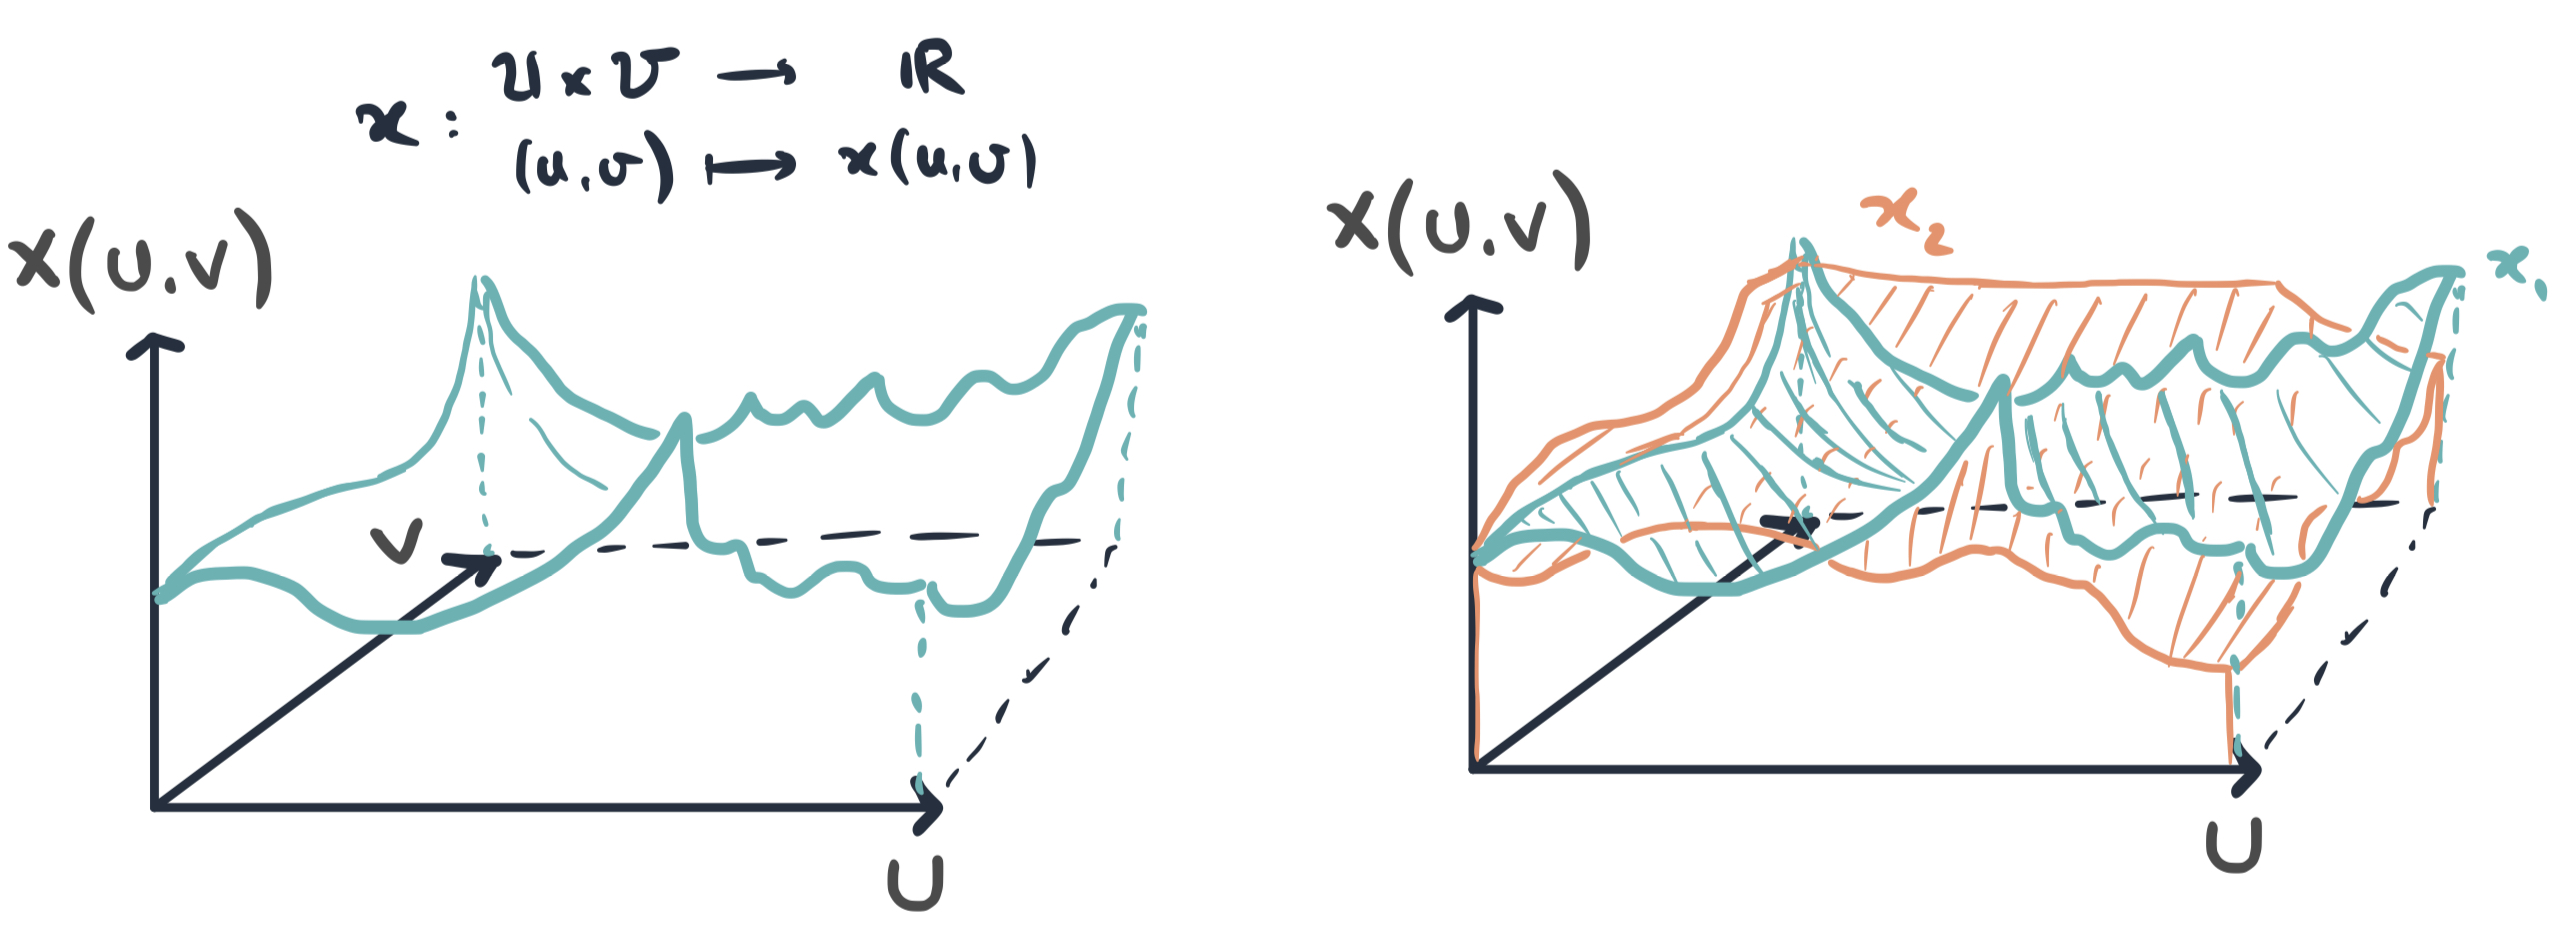
\includegraphics[width=0.8\textwidth]{Images/sketches/fda_surface.jpg}
	\end{center}

	{
	\textbf{Gauche :} exemple de surface
	\\
	\textbf{Droite :} échantillon de deux observations de la surface suivant une loi fonctionnelle}

	\caption{Donnée fonctionnelle : relation fonctionnelle avec plusieurs paramètres}
	\label{fig:sketch_surface}
\end{figure}

\noindent Maintenant introduites, les théorèmes suivant permettent de manipuler ces données à la fois pour la théorie et la pratique :

\begin{thm*}[\nameref{thm:KL} — informel]
	\noindent\fbox{%
		\parbox{\textwidth}{%
			Il est possible pour une large classe de données fonctionnelles de les décomposer dans une base \emph{de fonctions} adaptée aux données (au sens de la covariance) que l'on appelle base ACP fonctionelle (\textbf{FPCA}).
		}%
	}
	\label{thm*:KL}
\end{thm*}


\begin{rem}
	La classe de fonctions pouvant être décomposées est large, puisqu'elle regroupe l'ensemble des processus qui nous intéressent la plus part du temps en tant que statisticien : celles qui sont à support sur un intervalle, admettant une covariance continue et finie sur le support.
\end{rem}

On en déduit que pour travailler avec des données fonctionnelles, il suffit de les décomposer dans la base ACP fonctionnelle puis de travailler sur les composantes de chaque élément de la base. On travaille désormais avec des réels et non plus des fonctions, ce qu'on aime manipuler. On peut alors faire de la statistique traditionnelle avec les outils que l'on connait.


\begin{propriete*}[intérêt de la base FPCA — informel]
	\noindent\fbox{%
		\parbox{\textwidth}{%
			la base ACP fonctionnelle est la plus économe, c'est à dire qu'elle explique au mieux la covariance des données pour un nombre de composantes fixées, ce qui est utile car on ne sait manipuler numériquement que des objets de dimension finie.
		}%
	}
\end{propriete*}

Pour avoir une bonne représentation de ces données, on doit donc s'assurer de bien estimer la covariance. Pour cela, on a mentionné qu'il serait judicieux de lisser les observations en tenant compte de la régularité du processus dont sont issues nos données. La question est désormais la suivante :

\question{
	Est-il possible de récupérer la régularité locale des trajectoires à partir des données ? Si oui, comment ?
}

C'est ce qu'affirme le théorème suivant provenant des travaux de Golovkine et MPV :

\bigskip

% TODO : créer un alias samepage 
% \samepage{stuff} = \noindent\begin{minipage}{\textwidth} stuff \end{minipage}
\noindent\begin{minipage}{\textwidth}
\begin{thm*}[Regularité locale — informel]
	\noindent\fbox{%
		\parbox{\textwidth}{%
			Les données fonctionnelles permettent de récupérer la régularité locale des trajectoires. Les estimateurs définis \textbf{ponctuellement} convergent.
		}%
	}
	\label{thm*:regularite_locale}
\end{thm*}
\end{minipage}
\begin{rem}[Continuité de Kolmogorov]
	Un théorème (\nameref{thm:kolmogorov_continuite}) permet à partir de l'espérance d'incréments d'un processus aléatoire de déduire sa régularité.
	C'est pourquoi les estimateurs sont définis à partir des incréments quadratiques. C'est entre autres \emph{la raison pour laquelle les données fonctionnelles permettent de récupérer la régularité locale des trajectoires}.

	\label{rem:kolmo_continuite}
\end{rem}
